\clearpage
\section{Primer}

We start first by defining some common ideas, motives, and problems
within the scope of network topology modelling. 

\subsection{A Graph Primer}

In this context \define{topology} usually refers to the structure of
the \define{graph} representation of a network. That is, the common
notion used to describe network topology is the mathematical {\em
  graph}. \index{graph} A graph ${\cal G}$ is defined by a set of
nodes ${\cal N}$ (often called vertices) and edges (or links) ${\cal
  E} \subset {\cal N} \times {\cal N}$, so we usually write ${\cal G}
= ( {\cal N}, {\cal E})$.  Here, we shall denote the number of nodes
$N = |{\cal N}|$, and the number of edges $E = |{\cal E}|$.

Nodes are usually associated with some logical of physical structure
in a network: a router, switch, PoP, or AS. Edges are associated with
the appropriate type of logical or physical link between these nodes. 

A graph describes connectivity between logical resources such as
routers, or IP address, but simple connectivity is rarely as useful as
when additional information such as names, capacity or distance are
attached to these abstract objects. Such can easily be included in
these descriptions by creating labelling functions of the node or edge
sets, in the form: $f: {\cal N} \rightarrow \R$ or $f: {\cal E}
\rightarrow \R$ in the case of real-valued labels. We could similarly
defined labelling functions with text labels, or integer or vector
values, and so on. However, it is naive to treat labels as an
``add-on'' as they carry semantics that can be important in the
network. For instance, when we define link distances (be these
geographic or semantic), that can change the notion of distance in the
network as a whole.

We can also define functions of groupings of nodes or edges, though in
this case it is not as conceptually obvious why we might. However, an
exemplary case is that of ``on-net'' where we might define a function
that classifies pairs of nodes as on the same subnet or not. Thus,
such functions can ascribe meaning to groupings of nodes. 

Many of the Internet graphs have symmetric links (that is, if
$i\rightarrow j$ is a link, then $j \rightarrow i$ is also a link) and
so these networks are \define{undirected}, but we also need sometimes
to represent asymmetric links, and do so with a \define{directed
  graph} or \define{digraph}, and we call the links in such a digraph
\define{arcs}.

In the study of network topology we might come across the more
generalized graph concepts of the \define{multi-graph} and
\define{hyper-graph}. 
\begin{itemize}

  \item \define{hypergraph}: links connect more than two nodes
    \begin{itemize}
    \item \eg where you have a connective medium (rather than a
      wire), for instance in a wireless network.
    \end{itemize}

  \item \define{multigraph} or \define{pseudograph}: has multiple
    parallel links between two nodes
    \begin{itemize}
    \item \eg it is easy to have two links between two routers.
    \end{itemize}

\end{itemize}
We'll exclude these cases unless explicitly stated, but it is worth
noting that each of these do apply to particular aspects of the
Internet. 

We say two nodes are \define{connected} if a path exists between them,
and that a graph is connected if all pairs of nodes are connected. A
graph is $k-$node connected if the graph remains connected after the
removal of any set of $k-1$ or fewer nodes (and corresponding links)
and $k-$edge connected if the graph remains connected after the
removal of any $k-1$ edges.

For an undirected graph $G$, define the \define{neighborhood} of node
$i$ by
     \[ N_i = \big\{ j \mid (i,j) \in E \big\}, \]
\ie the set of adjacent nodes to $i$, and we define the degree of
the node to be  the number of elements in the neighborhood to be 
     \[ k_i = |N_i |. \]
In a directed graph, we define two concepts: the \define{in-degree}
(the number of links connecting to the link) and the
\define{out-degree} (the number of links originating from it). 
\begin{eqnarray*}
  \mbox{ \rm in-degree}(i) & = & \left|  \{ (j,i) | (j,i) \in
                                     {\cal E}  \}   \right|, \\
  \mbox{ \rm out-degree}(i) & = & \left| \{ (i,j) | (i,j) \in
                                     {\cal E}  \}   \right|.
\end{eqnarray*}
We often consider statistics of the degree distribution $p_k$ (which
gives the probability that a node has degree $k$), the average node
degree being the most obvious such. It can be easily calculated from
the sum of degrees, which has the interesting property
    \[ \sum_{i \in N} k_i = 2 |E|, \]
generally referred to the Handshake lemma. 

The node-degree distribution provides a common characterization of a
graph (though by no means a complete characterization).  It is
noteworthy, however, that although this distribution is frequently
discussed, the concept is somewhat ill-defined. It can be directly
measured for a real network, in which case $p_k$ is the probability
that a randomly selected node from the measured graph has degree
$k$. However, it is often used in the context of a set of simulated
graphs, where it is used to mean the probability that a node in the
ensemble of networks has degree $k$ with this probability. The
difference is subtle, but it is worth keeping track of such
discrepancies.

% Higher order statistics of the node degrees area also examined in some
% cases. In general, we might look at the ...

% However, there are some simple terms for some of these, perhaps the
% most noteworthy be \define{assortativity}, which is destined by 
% \[ r = \frac{\sum_{j,k} j k ( e_{j,k} - q_j q_k) }{\sigma^2_q},
% \]
% where $e_{i,j}$ is the fraction of edges that connect a vertex of type
% $i$ to one of type $j$, or the joint probability distribution of the
% remaining degree at either end of a randomly chosen link so
% $\sum_{j,k} e_{j,k} = 1$. We define $q_k$ by 
% \[ \sum_{j} e_{j,k} = q_k. 
% \] 
% $\sigma_q^2$

% For the statisticians, assortativity can be thought of as Pearson's
% correlation coefficient of remaining degrees at either ends of a
% random edge.

% Assortativity ranges from $-1$ to $1$ with the following meanings:
%   \begin{itemize}
%   \item $r$ near 1 -- high degree nodes often connect to high degree nodes,
%   \item $r$ near -1 -- high degree nodes often connect to low degree nodes.
%   \end{itemize}

% The above metrics are meaningful in the sense that they tell us the
% number of links per node, but often more important for engineers are
% distances. 

There are many other graph {\em metrics}. For instance, the
\define{distance}\footnote{The graph distance has a long history. In
  mathematics, perhaps the best known example is the Erd\H{o}s number,
  which is the distance of a author from Erd\H{o}s in the
  co-authorship graph. In popular culture there is an equivalent: the
  Bacon number, or the distance between actors in the graph of
  co-appearances.} between two connected nodes in an unweighted graphs
is generally defined to be the number of edges in the shortest path
connecting them. We can then examine quantities such as the average
distance, and the \define{diameter} of the network (the maximum
distance).

% Erd\H{o}s numbers: if you wrote a paper with Erd\H{o}s,
%   your number is 1. If you wrote a paper with a direct co-author, your
%   number is two, and so on. Essentially it is the graph distance you
%   are from Erd\H{o}s in a co-authorship graph.\\[2mm]

% \url{http://en.wikipedia.org/wiki/Erdos_number}\\[2mm]

% My Erd\H{o}s number is 4 (through Charles Pearce, Gavin Brown, and
% Robert Tijdeman.)\\[2mm]

% \url{http://www.ams.org/mathscinet/collaborationDistance.html}


  % \begin{itemize}

  % \item radius of a graph is the minimum eccentricity of any vertex
  %   \[ \mbox{radius}(G(N,E)) = \min_{i \in N} \epsilon(i). \]

  % \item diameter of a graph is the maximum eccentricity of any vertex
  %   \[ \mbox{diameter}(G(N,E)) = \max_{i \in N} \epsilon(i). \]
  %   which is the maximum distance between any pair of nodes.

  % \item a peripheral vertex is one whose eccentricity achieves the
  %   diameter.

  % \end{itemize}

And there are many other metrics: assortativity, clustering
coefficient, centrality, and so on. They are all attempts to capture
the nature of a graph in a small set of measures, and as such provide
simpler, seemingly more intuitive ways to consider graphs.  For other
discussions of these, and comparisons in the context of Internet
topologies see \cite{jamakovic08,haddadi08:_networ_topol}.  We must be
wary though, as it should be clear that the potential for problems is
immediate. No small set of numbers can truly represent graphs. For
instance, consider the Hamiltonian cycle\footnote{A Hamiltonian cycle
  is a path (on the graph) that visits each node exactly once, and
  then returns to the start point.} problem. The problem of
determining if a network has such a path is well known to be
NP-complete, and as such no small set of statistics of the graph will
provide a characterization that is sufficient to consider this
problem. Thus, these simple statistics must miss important properties
of the network.

% centrality
 
%   \begin{itemize}

%   \item Measures the ``centrality'' of a vertex in a graph

%   \item Different measures
%     \begin{itemize}
%     \item degree centrality (normalized degree) of nodes 
%       \begin{itemize}
%       \item interpretation --- how likely to catch a disease
%       \item extension to a metric on a graph (maximized by star)
%       \end{itemize}

%     \item closeness centrality 
%       \begin{itemize}
%       \item reciprocal of mean geodesic distance between $v$ and other nodes
%       \end{itemize}

%     \item between centrality
%       \begin{itemize}
%       \item normalized measure of how many shortest-paths a vertex
%         appears on
%       \end{itemize}

%     \end{itemize}

%   \end{itemize}

% clustering coefficient

%   \begin{itemize}

%   \item global measure of whether nodes tend to cluster
%   \[ c = 3 t_1 / t_2 , \]
% where
% \begin{eqnarray*}
%   t_1 & = & \mbox{number of triangles} \\
%   t_2 & = & \mbox{number of connected triples}
% \end{eqnarray*}

%   \item local measure of how close a node and its neighbors are to
%     being a clique
% \vspace*{-1mm}
% \[ c_i = \frac{\left| \{ (j,k)\in E | j,k \in N_i  \} \right|}{k_i  (k_i-1) /2}, \]
% where $N_i$ is the neighborhood of $i$, and $k_i=|N_i|$.

%   \end{itemize}

% $c_i$ counts the fraction of links in the local neighborhood, as
% compared with a clique.\\[2mm]

% we can compute a network average clustering co-efficient using
% \[ \bar{C} = \frac{1}{n} \sum_{i=1}^{n} c_i . \]



It may be useful to the reader to consider some of the tools that are
available for working with graphs. They have different sets of
feature, but perhaps the most important is whether they are used in
conjunction with a programming language and which one, so we have
listed a (no doubt incomplete) set below with some very basic
information.
  \begin{itemize}
\setlength{\itemsep}{-1mm}
\setlength{\topsep}{-1mm}

  \item MatlabBGL \url{http://www.stanford.edu/~dgleich/programs/matlab_bgl/}
    \begin{itemize}
    \item Graph libraries for Matlab, 
    \item using Boost Graph Library (BGL) \\
 {\url{http://www.boost.org/doc/libs/1_42_0/libs/graph/doc/index.html}}
    \end{itemize}

  \item igraph \url{http://igraph.sourceforge.net/}
    \begin{itemize}
    \item Libraries for working with graphs in R or Python
    \end{itemize}

  \item GraphVis \url{http://www.graphviz.org/}
    \begin{itemize}
    \item Toolkit for visualization of graphs
    \end{itemize}

  \item NetworkX \url{http://networkx.lanl.gov/}
    \begin{itemize}
    \item Python toolkit for working with graphs
    \end{itemize}

  \item GDToolkit
     \url{http://www.dia.uniroma3.it/~gdt/gdt4/index.php}
     \begin{itemize}
     \item OO C++ library for handling and drawing graphs
     \end{itemize}

  \item JUNG \url{http://jung.sourceforge.net/}
    \begin{itemize}
    \item Java universal network/graph framework
    \end{itemize}

  \item IGen \url{http://informatique.umons.ac.be/networks/igen/}
    \begin{itemize}
    \item A toolkit for generating IP network topologies based on
      network design heuristics. 
    \end{itemize}

  \end{itemize}

\subsection{Motivations for network topology investigations}

Underlying the whole research area is often an only vague notion of
why we study topology. The motives for such studies are in fact quite
diverse, and the implications are important. Topology studies
motivated by network managers with operational imperatives have
profoundly different requirements to those of the scientific research
community. Broadly speaking, we can divide the motivations as follows:
\begin{itemize}

\item {\bf Scientific:} Despite the fact that computer networks are
  designed (rather than grown as organic networks), little is known
  about their generic properties. Such knowledge would be useful
  (apart from satisfying simple curiosity) because there are many
  future protocols (for instance multicast protocols), and
  network-engineering algorithms (for instance see \cite{fortz00})
  whose design could benefit from an understanding of typical
  networks, rather than the typically very small, and unrealistic test
  examples often employed.

\item {\bf Adversarial:} Some network operators (though not all
  \cite{Zoo}) believe that commercial rivals might gain advantage
  through obtaining proprietary information about their network
  design. Similarly, there is a general belief that such information
  might facilitate an attack on the network. For instance, knowledge
  of a competitor's customers might be used by an adversary to target
  Denial of Service (DoS) attacks. One possible motivation for
  topology discovery is for just such an adversary to gain information
  to target attacks. 

\item {\bf Managerial:} It is often assumed that a network operator
  has a ``database of record'' that contains all the important
  information about their network. While this may be true in some
  cases, it is more often the case that such databases are hard to
  keep up-to-date and consistent with other data sources. This is
  actually a common problem in database
  management~\cite{dasu03:_data_mining}. Such databases must be
  maintained by humans, and as soon as they grow large, and complex
  (particularly when they are dynamic), it becomes exceedingly
  difficult to eradicate all human errors.  In addition, when the
  network undergoes change, particularly unplanned changes (failures),
  the database is unlikely to be accurate. Hence, for management of
  complex, dynamic networks, another source of data about the network
  is needed. It should be no surprise that obtaining this data from
  the network itself is the best solution for ensuring up-to-date,
  accurate records.

\item {\bf Informational:} This is a fairly general category of
  motivations, but differs from pure scientific curiosity in the
  immediacy of its application. For instance, customers of network
  operators often desire information about the networks to which they
  currently subscribe (in order to debug services, or obtain quality
  of service measurements), and also about networks to which they
  might subscribe (to help make choices about who could provide them
  with the most effective service). Often, a customer may not entirely
  trust its provider, or potential provider, and wish to verify
  information themselves. Hence, there is a need for such customers to
  be able to discover the networks to which they might subscribe, or
  where they should place services.

\end{itemize}
Each of these motivations imposes different requirements on our study
in terms of accuracy, immediacy, and the types of measurements
available. High degrees of accuracy are needed for network management;
and certainly the measurements used scientifically have rarely been
very accurate (though this is a significant problem with that
research). 

\subsection{Type of network}

The other core aspect we should consider is the type of topology to be
examined, as it can have a drastic affect on both observations and
behavior of the network. Two obvious dimensions are
\begin{description}
\item[Physical vs virtual:] Physical networks are built from hardware:
  routers and cables (copper or optical fiber for the Internet),
  transformers and cables for electricity, or cities and roads for the
  road network. Virtual networks may have physical nodes, but virtual
  edges (as in a social network), or virtual nodes and edges (as in
  online social networks, or the WWW). 

  The main difference is that there are usually large costs in
  building, or adding to a physical network. Virtual networks, on the
  other hand, have much smaller costs (an HTML link costs almost
  nothing to create). Costs have a profound affect on network designs,
  as we shall later see, but also on dynamic behavior. If it is
  easier to change a network, it can change more quickly.

  The other major issue for a physical network is that it is often
  bound by physical constraints, and this also profoundly affect their
  design.

  \autoref{fig:phys_v_virt} illustrates the differences, and also makes the point
  that it isn't really a binary difference. Networks lie on a spectrum.

\begin{figure}[htp]
  \begin{center}
    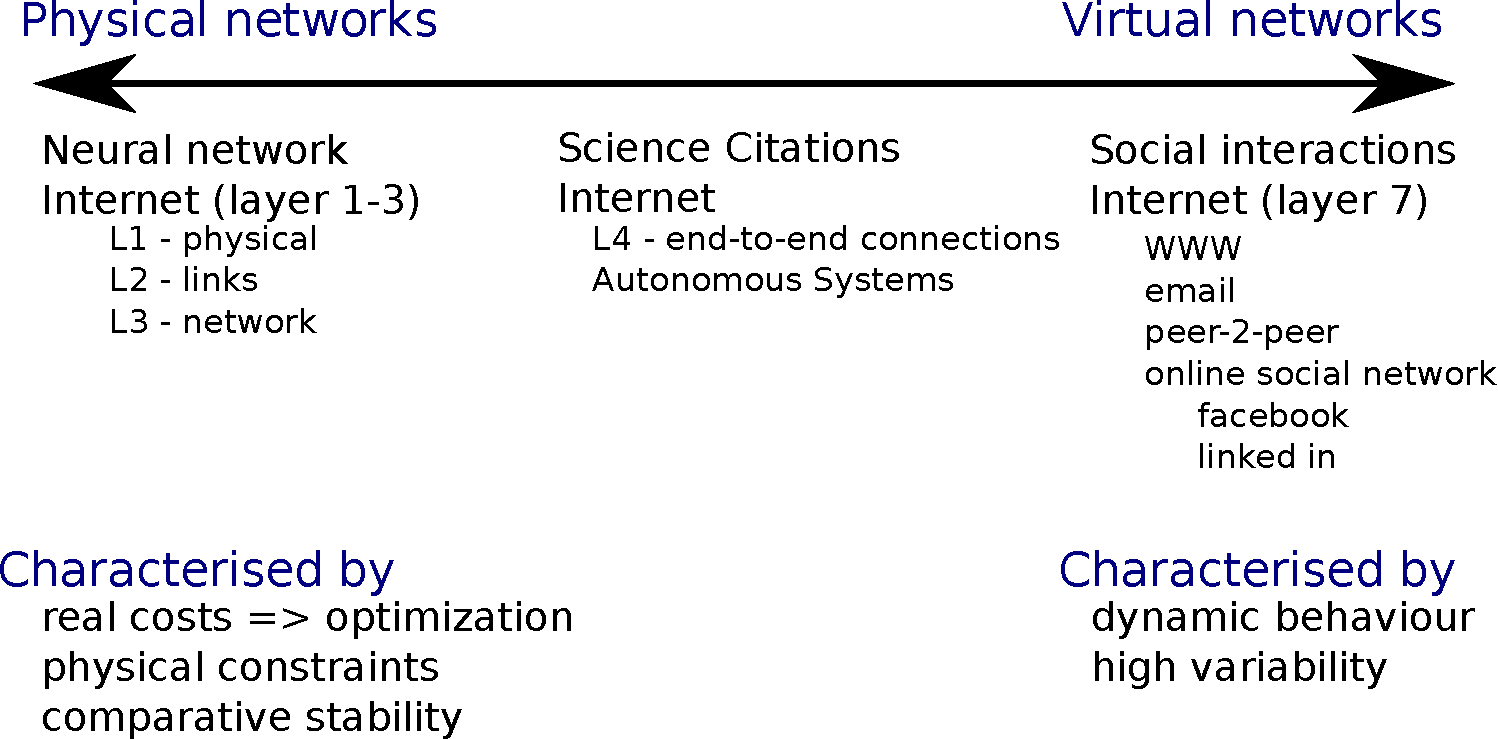
\includegraphics[width=1.1\figurewidth]{physical_vs_virtual.pdf}
    \caption{Physical vs virtual networks.\label{fig:phys_v_virt}}
  \end{center} 
\end{figure}


\item[Transport vs Information flows:] A more subtle differentiator
  is between what the network carries. Some networks physically
  transport some type of material (cars, water, ...) whereas the flows
  in other networks are (almost) pure information (the Internet,
  ...).  

  The importance of this distinction for networks may be less
  immediately obvious, but it certainly does have implications. When
  physical transport is involved in a network, the constraints on that
  network are likely to be even more stringent, and the ability to
  change the network even more limited. Costs for changing the road
  network, for instance, are usually higher than changing the
  equivalent proportion of a IP network.

\begin{figure}[htp]
  \begin{center}
     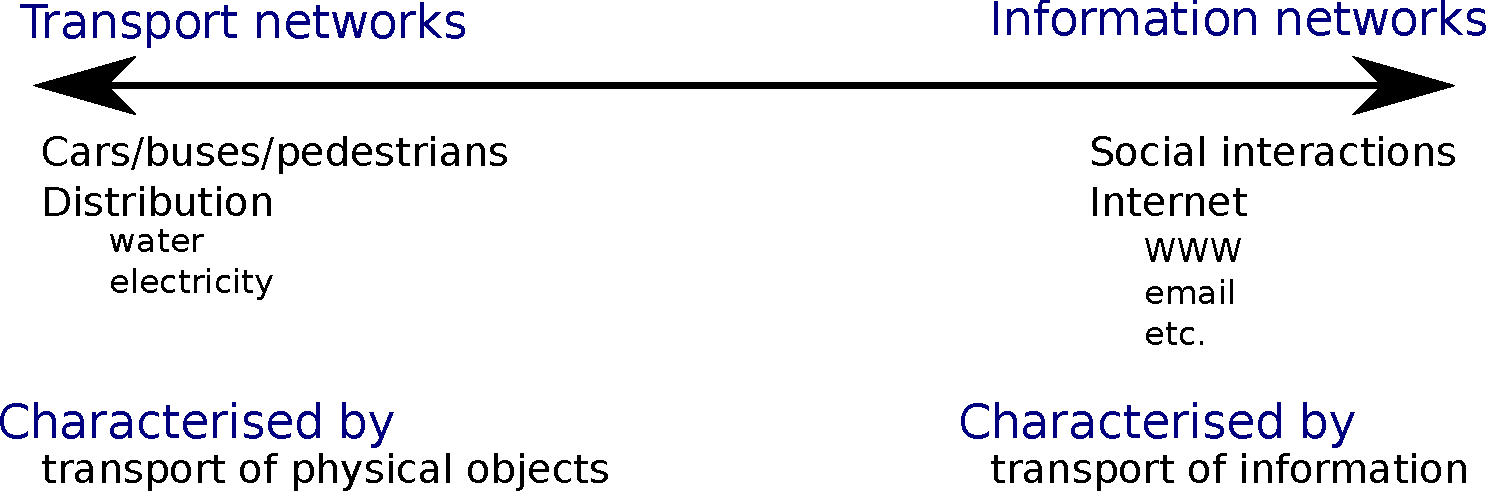
\includegraphics[width=1.1\figurewidth]{physical_vs_information.pdf}
 
    \caption{Transport vs information flows.\label{fig:trans_v_inf}}
  \end{center}
\end{figure}         

\end{description}
Within this chapter, we are primarily interested in the ``Internet'',
and that includes both physical (OSI layer 1-3) networks, and virtual
networks (MPLS, WWW, online social networks, etc.). However, all of
the networks considered here are information transportation networks.

There are other dimensions on which networks could be classified. For
instance, by the nature of the transport. Does it come in discrete
chunks (\eg cars, packets, or the post) or continuously (\eg water or
electricity)? Is the transport connection oriented (\eg the telephone
network) or packet oriented (\eg the Internet)?

And there are other general issues we need to deal with:
\begin{itemize}

  \item Physical networks are embedded in geography, but logical
    networks often aren't, and yet the same terminology is often
    applied to each.

  \item Connectivity often changes over time, with the time-scale
    varying depending on the type of network.

  \item The Internet is often said to be a ``network of networks''. It
    is often hard to consider one network in isolation, they have
    relationships, but the situations is even more complicated than
    often imagined.
    \begin{description}

    \item[peers] Networks may be connected to {\em peers}, \ie similar
      networks that may be competing or co-operating (or both in some
      cases), \eg two ISPs operating in the same region.

    \item[parents] Networks may have a parent-child relationship in
      the sense that one network controls the other, \eg the SS7
      network with respect to traditional telephone network.

    \item[layers] A single network may have multiple layers, each of
      which can be represented by a different graph, \eg the physical-
      vs the network-layers in the Internet.

    \item[external] There is substantial interaction between
      notionally separated networks, \eg the power grid and the
      Internet, both because the Internet uses electricity, but also
      because spikes in electricity demand could potentially be caused
      by network flash crowds (certainly TV programs have a very
      important impact on electricity usage).

    \end{description}
    
\end{itemize}

That brings us naturally to the particular object of discussion here
-- the Internet (and its topology).  The term ``Internet'' means
(many) different things to (many) different people.  Even within the
networking community, the term is often used ambiguously, leading to
misunderstandings and confusion and creating roadblocks for a
genuinely scientific treatment of an engineered system that has
revolutionized the way we live.

While mathematics in the form of graph theory has been equally
culpable in adopting the use of this vague nomenclature, the ``new
science of networks'' has popularized it to the point where phrases
like ``topology of the Internet'' or ``Internet graph'' have entered
the mainstream science literature, even though they are essentially
meaningless without precisely-stated definitions.  For one, ``Internet
topology'' could refer to the connectivity structures encountered in
any of layers in the protocol stack, or at various levels of
aggregation. Common examples are
\begin{enumerate}

\item {\bf Router-level (layer 3):} An often sought topology is the
  router level. Somewhat ambiguously, this may also be called the
  network level, or IP level, but ``network'' is a heavily overloaded
  term here, and the IP level can also be ambiguous. For instance, IP
  level could refer to the way IP addresses are connected, that is it
  could refer to the interfaces of one router as separate nodes
  \cite{broido01:_inter}, but that is rarely what is useful for
  network operations or research. We could also add at layer 3, in
  addition to {\em interface-level} topology described above, the {\em
    subnet-level} topology
  \cite{kardes12:_cheleb,gunes09:_resol_ip_inter,Tozal:2012:ENL:2342042.2342069,Tozal:tracenet:imc2010,broido01:_inter},
  describing the interconnectivity of logical subnets (often described
  by an IP-level prefix), but here we focus on the more commonly
  considered router level.

  The router-level graph shows a range of interesting implementation
  details of a network. This type of information is critical for
  network management applications, as much of Internet management
  rests at the IP layer, and it is of great importance for network
  adversaries. For instance, developing tools to measure network
  traffic requires an understanding of the router-layer topology, in
  order to match traffic to links. Similarly traffic engineering, and
  reliability analyses are carried out at this level. One complication
  of this layer is that we sometimes wish to obtain the topology
  extending out to end-hosts, which are not technically routers, but
  we shall include these in our definition of router-layer topology,
  unless otherwise specified.

\item {\bf Switch-level (layer 2):} A single IP layer logical link may
  hide several layer-2 devices (hubs and switches). The increasing
  prevalence of Ethernet, and the ability to provide redundancy at
  reasonable cost, has led to a proliferation of such devices, and
  most Local Area Networks (LANs) are based around such. Hence, very
  many networks which have trivial, or simple IP layer topologies have
  complex and interesting layer-2 topologies. Multi-Protocol Label
  Switching (MPLS) further complicates the situation by creating
  logical layer-2 networks without physical devices, often in the form
  of cliques. Measurements often see only one layer, creating
  misunderstandings of a network's true resilience and more general
  graph properties. For instance, layer-2 devices can connect large
  numbers of routers, making them appear to have higher degree at
  layer-3 \cite{Merindol:layer2:imc2010} (for more detailed discussion
  see \autoref{sec:mpls}).

\item {\bf Physical-level (layer 1):} Below the link layer (layer 2),
  lies the physical layer. Again, many physical devices may underly a
  single logical link. Discovery of this layer is of critical
  importance in network management tasks associated with
  reliability. In particular, the concept of Shared Risk Link Groups
  (SRLG) requires knowledge of which links are carried on which fibers
  (using Wavelength Division Multiplexing), in which conduits. If a
  backhoe digs up a single conduit, it will cause a bundle of fibers
  to fail, and so connections that are in the same SRLG will all fail
  simultaneously. Clearly redundant links need to be in different
  SRLG, and discovery of the physical topology is important to ensure
  that this is the case.

\item {\bf PoP-level:} A Point-of-Presence (PoP) is a loosely defined
  grouping of devices, often defined by a metropolitan area.  PoP
  level topologies are quite useful, essentially because these graphs
  describe the logical structure of the network as the designer
  intended, rather than its particular implementation in terms of
  individual routers. Such topologies are ideal for understanding
  tradeoffs between connectivity and redundancy, and also provide the
  most essential information to competitors or customers (about where
  a network is based, or who has the best access network in a
  region). Network maps are often drawn at this level because it is an
  easy level for humans to comprehend.

\item {\bf Application layer:} There has been significant interest in
  logical topologies of the application layer, \eg for the Web
  (using HTTP, and HTML), and the P2P applications. 
% We will not
%   consider such topologies in any detail here. Some approaches may be
%   similar, but by and large the approaches to determining these
%   topologies are very application dependent, \eg web crawlers for the
%   WWW.

\item {\bf AS-level:} AS topologies have generated much interest in
  the scientific literature~\cite{barabasi99,barabasi00,barabasi02},
  because they appear to show interesting properties (such as
  power-laws) in common with other un-engineered networks such as
  biological networks. Also, much data on AS topologies is publicly
  available. While of interest in the scientific literature, this
  data's use is confused by many myths and
  misunderstandings~\cite{roughan11}.  The data may provide mild
  competitive benefits, in allowing operators to determine who peers
  with who, but the measured data often comes without attributes that
  would make the data truly useful in this regard. Finally, it is hard
  to see how such data could be used in an attack, although much
  publicized reports such as \cite{barabasi02} suggest, incorrectly
  (see \cite{Li04}), that the observed structure of the AS graph may
  lead to an ``Achilles heel'' of the Internet.

  % \item {\bf Others:} There are other topologies that may be of
  % interest from time to time, for instance, that of a multicast
  % tree. 

\end{enumerate}
The number of possible topologies we might wish to discover highlights
the complexity of this problem, and why discovery is so valuable for
network management. In this chapter we will consider the router-level
topology in detail, and then discuss some of the similarities and
differences with respect to AS- and PoP-level topologies.

In addition to understanding the Internet network as a simple graph,
there are many other features of the graph that one would also wish to
know, for instance, its routing, link capacities, and geographic
locations. We describe such qualities as graph attributes, and find
that most can either be attributed to edges of the graph, for instance
\begin{sitemize} 

  \item link capacities,

  \item link length,
 
  \item routing weights (\eg for shortest-path routing),

  \item link utilizations,

  \item link performance (for example, bit-error-rate, delay, loss,
  jitter, reordering, buffer utilization), 

  \item link status (up/down), and 

  \item a link's lower layer properties (\eg number of physical hops),

\end{sitemize}
or to the nodes of the graph
\begin{sitemize}

  \item geographic location,

  \item type of node, \eg brand of router, or version of software,

  \item performance measures (\eg CPU utilization), and 

  \item node status (up/down).

\end{sitemize}
We could further divide this list into \define{intrinsic} network
properties, such as node location, or link capacity (things that
cannot change easily), and \define{extrinsic} properties, such as
performance, or traffic related properties, which can change
dramatically despite there being no change in the underlying network.

% In a few cases, it is hard to attribute a quality to an individual
% component of the network. For instance, routing in a network is often
% of interest. In the case of shortest path routing, this can be
% completely characterized by simple link weight attributes for each
% link, but many networks use routing protocols to create more complex
% routings. This type of complexity can sometimes be simply described by
% simple attributes, but may in other cases may be rather more
% difficult. For example OSPF with areas is often used to create a type
% of hierarchy within an AS --- in this example we can still use link
% attributes because we can assign an OSPF area to each link, but the
% attributes may be more difficult to measure. In other cases, for
% example if BGP was used as an IGP to create policy based routing
% internally in a network, we cannot describe the routing with simple
% attributes (to some extent the routing could still be captured by the
% forwarding table, which is an extreme example of a router attribute,
% but we shall exclude such extreme cases of attributes for the
% moment.). In these cases, the attributes really belong to end-to-end
% paths through the network, keyed on IP addresses (source and
% destination). We shall not consider such attributes in this report,
% though they may be of interest.

%% As an example of how one might use attributes: given node locations, it
%% is trivial to build a PoP level topology from a router-level topology.

